\documentclass{article}
\usepackage{amsmath}
\usepackage{amssymb}
\usepackage{graphicx}
\usepackage{hyperref}
\usepackage[version=4]{mhchem}

\title{Example 12}
\date{}

\begin{document}
\maketitle

\(\triangle A B C\) is an isosceles right triangle with \(\angle A=90^{\circ}\). Points \(P\) and \(Q\) are points on sides \(A B\) and \(A C\), respectively. \(B P=A Q\). Show that \(\triangle P D Q\) is also an isosceles right triangle if \(D\) is the midpoint of \(B C\).

Solution:
Draw the median \(A D\).\\
Since \(\triangle A B C\) is an isosceles right triangle and \(D\) is the midpoint of \(B C, A D \perp B C, \angle A D C=90^{\circ}\).\\
By Theorem 1.3, \(A D=B D=D C . \angle D A Q=\angle A=45^{\circ}\).\\
\centering
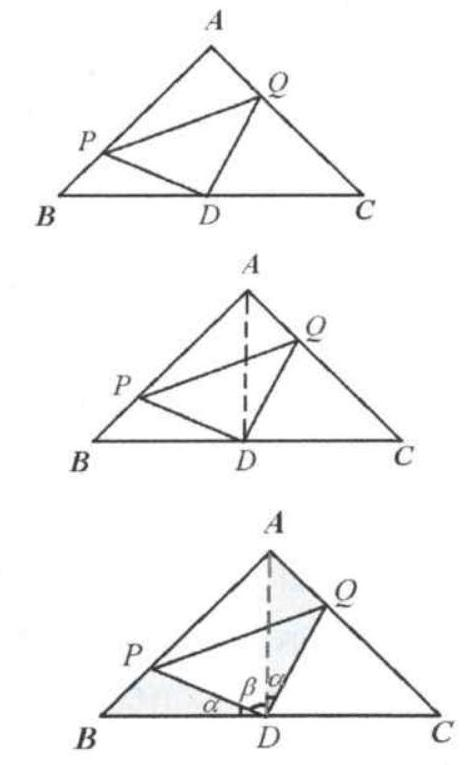
\includegraphics[width=\textwidth]{images/013(1).jpg}

Since \(B P=A Q, \triangle B P D \cong \triangle A Q D\).\\
Thus, \(P D=Q D . \angle A D Q=\angle B D P=\alpha\).\\
We see that \(\angle A D Q=\alpha+\beta=90^{\circ}\).\\
So \(\angle P D Q=\alpha+\beta=90^{\circ}\).

We also know that \(P D=Q D\).\\
Thus \(\triangle P D Q\) is an isosceles right triangle.



\end{document}
